\documentclass[a4paper,12pt]{article}
\usepackage{amsmath,amssymb}
\usepackage{graphicx}
\usepackage{scaladefs}
\usepackage{scalit}
\usepackage{fancyhdr}
\pagestyle{fancy}
\lhead{\today}
\rhead{markup/markup.nw}
\begin{document}
\section{The noweb markup format}
While the final goal of the literate programming tools is to extract the
source and documentation from a \texttt{noweb} file, we will not work with the
raw input source, but with an intermediary format called \texttt{markup}, where
the function of each line is explicitly noted. The following classes will
convert a \texttt{noweb} file into a marked up file.

After we have converted the input from this format (or after we have
directly read the intermediate format), another stage will convert our
stream of lines in a stream of blocks. Only this format will then be used
for \texttt{tangle} which generates the code and \texttt{weave} which generates
the documentation.

The next graphic illustrates the stages that we will go through:

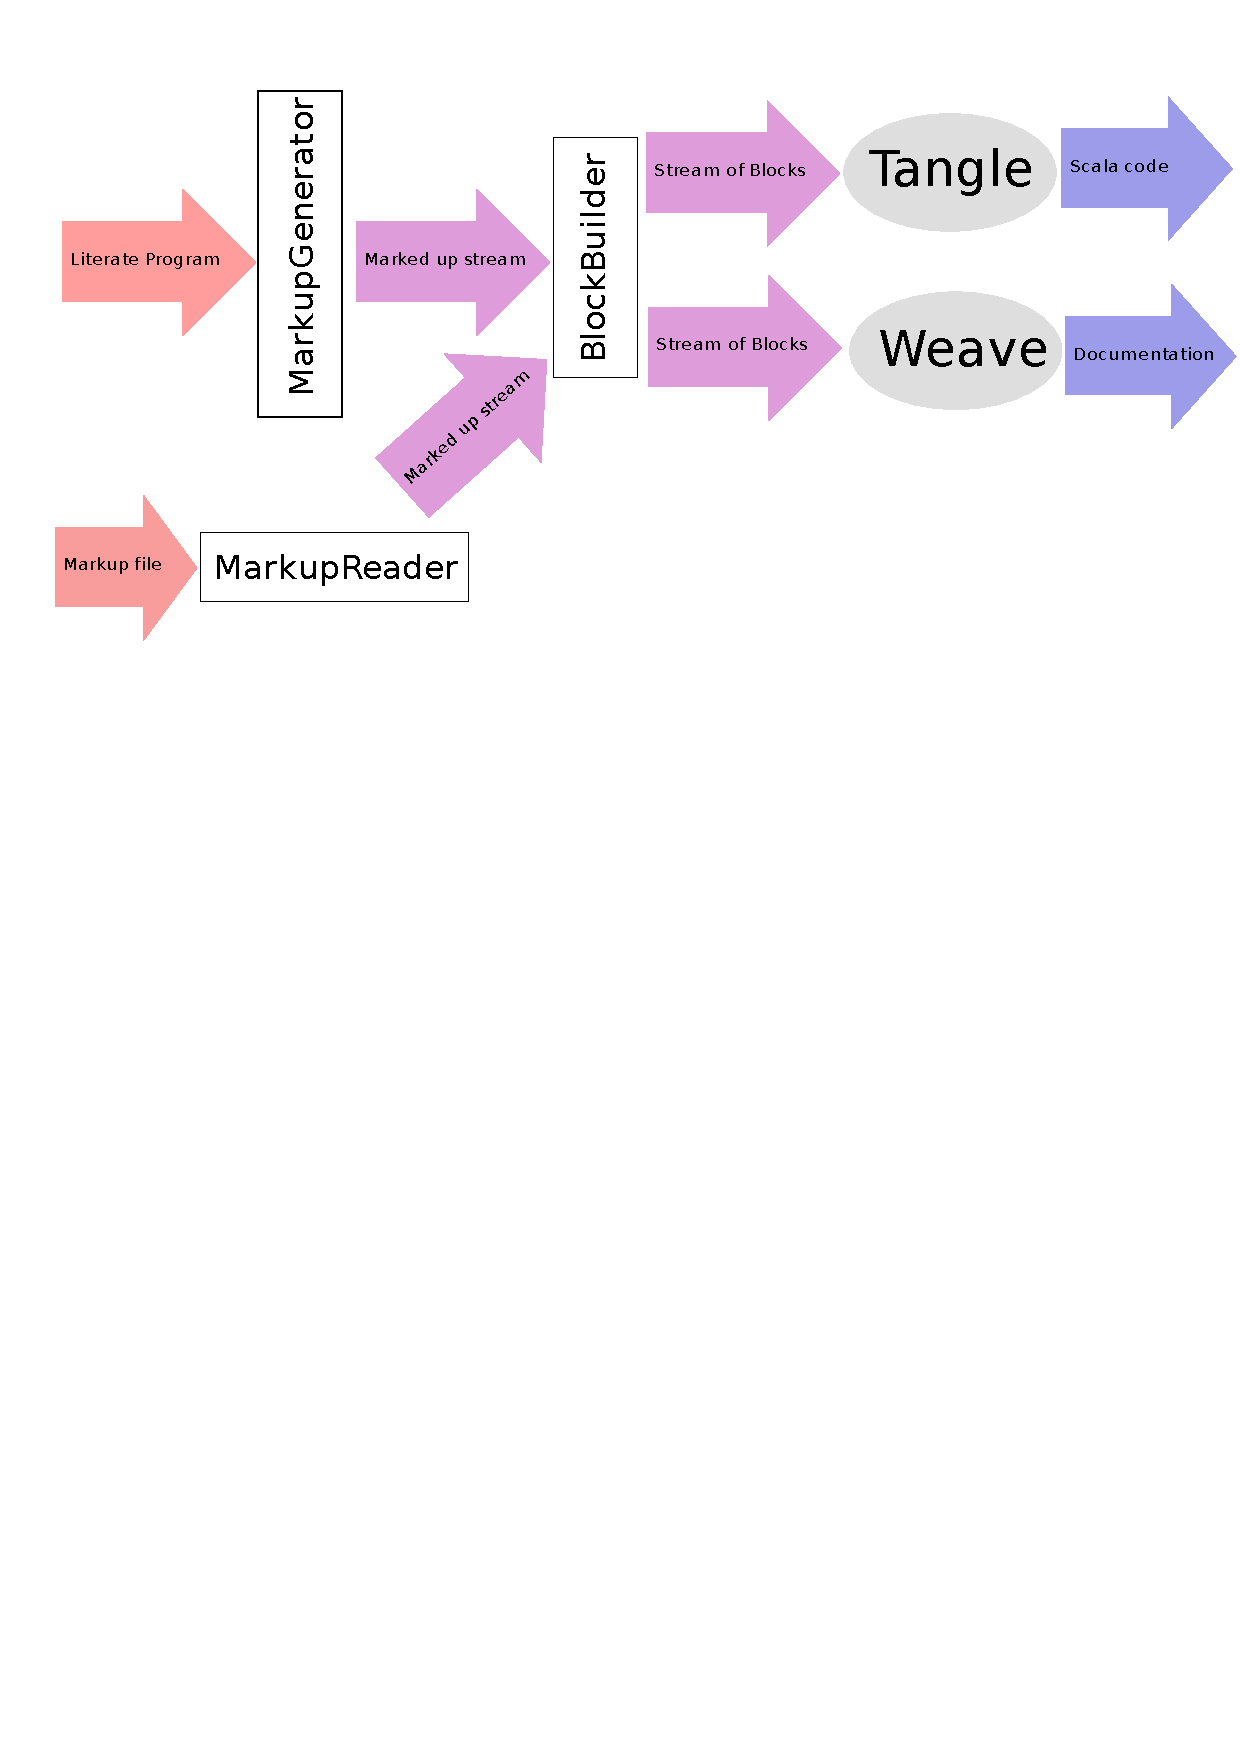
\includegraphics[width=16cm,viewport=0 550 800 800]{images/overview}

\subsection{Outline}
The Noweb markup that we will use is very light and only consists of
very few different cases, however, they all interact, so the conversion
part is still quite difficult. A noweb file will contain:

\begin{itemize}
\item source chunks (whose beginning is indicated by an @ sign)
\item quoted text (indicated by \texttt{[[} and \texttt{]]})
\item code chunks between \texttt{$\langle$$\langle$} and \texttt{$\rangle$$\rangle$=}
\item use directives (also between \texttt{$\langle$$\langle$} and \texttt{$\rangle$$\rangle$}, but without an =
afterwards
\end{itemize}

More details of the format can be found in the file \texttt{markup.nw} in the
noweb distribution\footnote{Noweb home page: http://www.eecs.harvard.edu/nr/noweb/}

This will then be converted in the intermediary format. To get a rough feeling for
the intermediary format, we will first treat this format and write the conversion
classes to this intermediary format afterwards:

$\left<\mbox{\emph{*}}\right>\equiv$
\begin{program}{\vem package}~scalit.markup
\\[0.5em]$<$line~types$>$
\\[0.5em]$<$read~in~the~intermediary~format$>$
\\[0.5em]$<$markup~reader$>$
\\[0.5em]$<$conversion~from~noweb~to~markup$>$
\\[0.5em]$<$markup~generator$>$
\\[0.5em]\end{program}


\subsection{The line types of the intermediary format}
There are about a dozen different line types. Let us first define these
line types and then consider how to read in a file in this format.

$\left<\mbox{\emph{line types}}\right>\equiv$
\begin{program}{\vem abstract}~{\vem class}~Line
\\[0.5em]\end{program}\classdefinition{Line}



Now for the subclasses

\begin{description}
\item[A line of text] Might occur inside documentation chunks but also
inside code chunks.

$\left<\mbox{\emph{line types}}\right>+\equiv$
\begin{program}{\vem case}~{\vem class}~TextLine$($content\,{\rm :}~String$)$~{\vem extends}~Line~{\small\{}
\\~~~~{\vem override}~{\vem def}~toString~=~"@text~"~$+$~content
\\{\small\}}
\\[0.5em]\end{program}\classdefinition{TextLine}
\methoddefinition{TextLine}{toString}
\valuedefinition{TextLine}{content }



\item[A new line] Because we will be splitting up one line in different lines
describing the structure of the file, we will have to indicate when a newline
character occured in the source file. This is done with the following class:

$\left<\mbox{\emph{line types}}\right>+\equiv$
\begin{program}{\vem case}~{\vem object}~NewLine~{\vem extends}~Line~{\small\{}
\\~~~~{\vem override}~{\vem def}~toString~=~"@nl"
\\{\small\}}
\\[0.5em]\end{program}\objectdefinition{NewLine}
\methoddefinition{NewLine}{toString}



\item[Quotes] Section of the text will be quoted and will appear verbatim
in the documentation. They are situated betwen beginning and end quote tokens:

$\left<\mbox{\emph{line types}}\right>+\equiv$
\begin{program}{\vem case}~{\vem object}~Quote~{\vem extends}~Line~{\small\{}
\\~~~~{\vem override}~{\vem def}~toString~=~"@quote"
\\{\small\}}
\\{\vem case}~{\vem object}~EndQuote~{\vem extends}~Line~{\small\{}
\\~~~~{\vem override}~{\vem def}~toString~=~"@endquote"
\\{\small\}}
\\[0.5em]\end{program}\objectdefinition{Quote}
\objectdefinition{EndQuote}
\methoddefinition{Quote}{toString}
\methoddefinition{EndQuote}{toString}



\item[Code chunks] Like quotes, we will designate code chunks by their
beginning and end. Another important information will be the \emph{number} of
this chunk: Code and documentation chunks are numbered consecutively.

$\left<\mbox{\emph{line types}}\right>+\equiv$
\begin{program}{\vem case}~{\vem class}~Code$($number\,{\rm :}~Int$)$~{\vem extends}~Line~{\small\{}
\\~~~~{\vem override}~{\vem def}~toString~=~"@begin~code~"~$+$~number
\\{\small\}}
\\{\vem case}~{\vem class}~EndCode$($number\,{\rm :}~Int$)$~{\vem extends}~Line~{\small\{}
\\~~~~{\vem override}~{\vem def}~toString~=~"@end~code~"~$+$~number
\\{\small\}}
\\[0.5em]\end{program}\classdefinition{Code}
\classdefinition{EndCode}
\methoddefinition{Code}{toString}
\methoddefinition{EndCode}{toString}
\valuedefinition{Code}{number }
\valuedefinition{EndCode}{number }



As already mentioned, code chunks will be given names so that they
can be used as part of other code chunks. This information will be the
first line inside a code section:

$\left<\mbox{\emph{line types}}\right>+\equiv$
\begin{program}{\vem case}~{\vem class}~Definition$($chunkname\,{\rm :}~String$)$~{\vem extends}~Line~{\small\{}
\\~~~~{\vem override}~{\vem def}~toString~=~"@defn~"~$+$~chunkname
\\{\small\}}
\\[0.5em]\end{program}\classdefinition{Definition}
\methoddefinition{Definition}{toString}
\valuedefinition{Definition}{chunkname }



Now that we have a line indicating which code chunk is defined, we can
also envisage to use it in other code chunks:

$\left<\mbox{\emph{line types}}\right>+\equiv$
\begin{program}{\vem case}~{\vem class}~Use$($chunkname\,{\rm :}~String$)$~{\vem extends}~Line~{\small\{}
\\~~~~{\vem override}~{\vem def}~toString~=~"@use~"~$+$~chunkname
\\{\small\}}
\\[0.5em]\end{program}\classdefinition{Use}
\methoddefinition{Use}{toString}
\valuedefinition{Use}{chunkname }



\item[Documentation] Like code chunks, documentation chunks will be given
a number. Otherwise, they behave the same:

$\left<\mbox{\emph{line types}}\right>+\equiv$
\begin{program}{\vem case}~{\vem class}~Doc$($number\,{\rm :}~Int$)$~{\vem extends}~Line~{\small\{}
\\~~~~{\vem override}~{\vem def}~toString~=~"@begin~docs~"~$+$~number
\\{\small\}}
\\{\vem case}~{\vem class}~EndDoc$($number\,{\rm :}~Int$)$~{\vem extends}~Line~{\small\{}
\\~~~~{\vem override}~{\vem def}~toString~=~"@end~docs~"~$+$~number
\\{\small\}}
\\[0.5em]\end{program}\classdefinition{Doc}
\classdefinition{EndDoc}
\methoddefinition{Doc}{toString}
\methoddefinition{EndDoc}{toString}
\valuedefinition{Doc}{number }
\valuedefinition{EndDoc}{number }



\item[Special indicators] We will have two special indicators: One telling us
which file we are reading and one to indicate the end of our input.

$\left<\mbox{\emph{line types}}\right>+\equiv$
\begin{program}{\vem case}~{\vem class}~File$($filename\,{\rm :}~String$)$~{\vem extends}~Line~{\small\{}
\\~~~~{\vem override}~{\vem def}~toString~=~"@file~"~$+$~filename
\\{\small\}}
\\{\vem case}~{\vem object}~LastLine~{\vem extends}~Line
\\[0.5em]\end{program}\classdefinition{File}
\objectdefinition{LastLine}
\methoddefinition{File}{toString}
\valuedefinition{File}{filename }



\end{description}

To test whether the intermediary format was completely described, we
will build a small parser for it in the next section.

\subsection{Reading in the intermediary format}

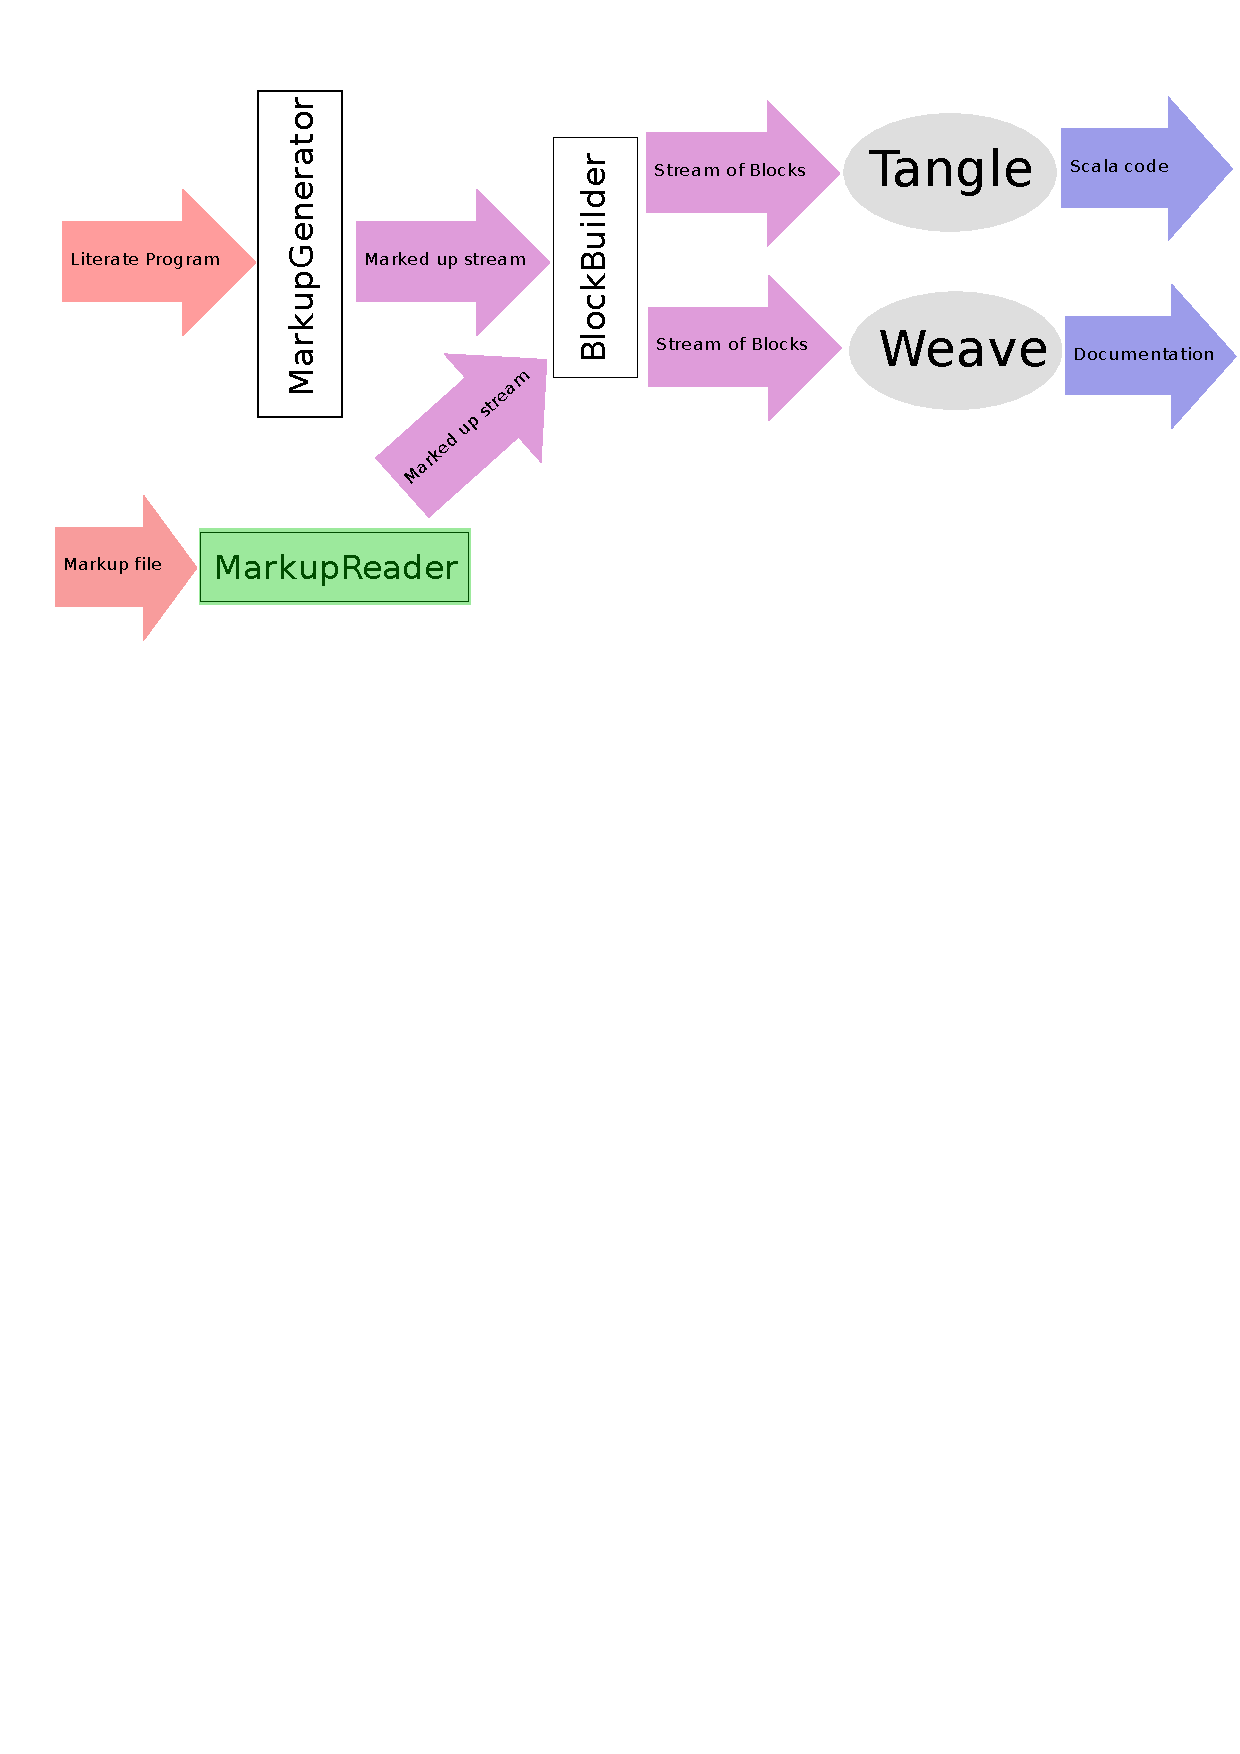
\includegraphics[viewport=0 500 264 800,clip,height=7cm]{images/markupReader.pdf}

A parser for the intermediary format will be much simpler than the one
we will have to build for the noweb source format: It suffices to parse
the beginning of a line to get the function. This simple parser will
consist of two methods, one that gets the next token and one that
represents all the tokens of a file as a stream.

$\left<\mbox{\emph{read in the intermediary format}}\right>\equiv$
\begin{program}{\vem import}~scala.util.parsing.input.StreamReader
\\{\vem class}~MarkupParser$($in\,{\rm :}~StreamReader$)$~{\small\{}
\\~~~~$<$get~next~token~of~markup~file$>$
\\~~~~$<$token~stream~of~markup~file$>$
\\{\small\}}
\\[0.5em]\end{program}\classdefinition{MarkupParser}
\valuedefinition{MarkupParser}{in}



Note that the MarkupParser takes a stream reader representation of
the input file as constructor argument. With a StreamReader, we have
the possibility to record our position in the file while reading.

Let us first look at the stream representation: We know we have read the
last token when we see \texttt{LastLine}

$\left<\mbox{\emph{token stream of markup file}}\right>\equiv$
\begin{program}{\vem def}~lines\,{\rm :}~Stream$[$Line$]$~=~{\small\{}
\\~~~~{\vem def}~lines0$($input\,{\rm :}~StreamReader$)${\rm :}~Stream$[$Line$]$~=
\\~~~~nextToken$($input$)$~{\vem match}~{\small\{}
\\~~~~~~~~{\vem case}~$($LastLine,rest$)$~$\Rightarrow$~Stream.empty
\\~~~~~~~~{\vem case}~$($line,rest$)$~$\Rightarrow$~Stream.cons$($line,~lines0$($rest$)$$)$
\\~~~~{\small\}}
\\~~~~lines0$($in$)$
\\{\small\}}
\\[0.5em]\end{program}\methoddefinition{MarkupParser}{lines}



After we have read the token, we will have advanced in the stream, therefore
we will read in the next token from the returned position.

This stream representation will be quite useful when we are processing
the input with tangle and weave. But let us move on to the method that
actually gives us the token:

$\left<\mbox{\emph{get next token of markup file}}\right>\equiv$
\begin{program}{\vem def}~nextToken$($input\,{\rm :}~StreamReader$)${\rm :}~$($Line,StreamReader$)$~=~{\small\{}
\\~~~~{\vem def}~readLine$($inreader\,{\rm :}~StreamReader,
\\~~~~~~~~~~~~~~~~~~~~~~acc\,{\rm :}~List$[$Char$]$$)${\rm :}~$($List$[$Char$]$,StreamReader$)$~=
\\~~~~~~~~{\vem if}$($~inreader.atEnd~$\,|$$\,|$~inreader.first~$==$~'$\backslash$n'~$)$
\\~~~~~~~~~~~~$($inreader.first~{\rm :}{\rm :}~acc.reverse,~inreader.rest~$)$
\\~~~~~~~~{\vem else}~readLine$($inreader.rest,~inreader.first~{\rm :}{\rm :}~acc~$)$
\\[0.5em]\end{program}\methoddefinition{MarkupParser}{nextToken}



This little function reads in the whole line and returns the position
afterwards.

$\left<\mbox{\emph{get next token of markup file}}\right>+\equiv$
\begin{program}~~~~in.first~{\vem match}~{\small\{}
\\~~~~~~~~{\vem case}~'@'~$\Rightarrow$~{\small\{}
\\~~~~~~~~~~~~{\vem val}~$($line,rest$)$~=~readLine$($input.rest,Nil$)$
\\~~~~~~~~~~~~{\vem val}~directive~=~$<${\vem match}~on~the~directive~to~produce~the~line$>$
\\~~~~~~~~~~~~$($directive,rest$)$
\\~~~~~~~~{\small\}}
\\~~~~~~~~{\vem case}~\_~$\Rightarrow$
\\~~~~~~~~~~~~System.err.println$($"Found~a~line~not~beginning"~$+$
\\~~~~~~~~~~~~~~~~~~~~~~~~~~~~~~~~~~"~{\vem with}~@,~but~{\vem with}~"~$+$
\\~~~~~~~~~~~~~~~~~~~~~~~~~~~~~~~~~~input.first$)$
\\~~~~~~~~~~~~exit$($1$)$
\\~~~~{\small\}}
\\{\small\}}
\\[0.5em]\end{program}


When having read a line, we take the directive which is everything before
the first space character. So we split along the spaces. However, strangely
enough the readLine function (and therefore StreamReader) seems to insert
a strange character at the beginning (this might as well be a bug), so we will
have to continue after that.

$\left<\mbox{\emph{match on the directive to produce the line}}\right>\equiv$
\begin{program}$($line.tail~mkString~""~split~'~'$)$.toList~{\vem match}~{\small\{}
\\~~~~{\vem case}~"file"~{\rm :}{\rm :}~sth~$\Rightarrow$~File$($sth~mkString~"~"$)$
\\[0.5em]\end{program}


The file line has one more argument: The filename. We thus simply reconstruct
it from the argument list.

After the file token, we will usually find a beginning of either a code or
a documentation chunk. The only argument this takes is the chunk number.

$\left<\mbox{\emph{match on the directive to produce the line}}\right>+\equiv$
\begin{program}~~~~{\vem case}~"begin"~{\rm :}{\rm :}~"docs"~{\rm :}{\rm :}~number~{\rm :}{\rm :}~Nil~$\Rightarrow$
\\~~~~~~~~Doc$($Integer.parseInt$($number$)$$)$
\\~~~~{\vem case}~"begin"~{\rm :}{\rm :}~"code"~{\rm :}{\rm :}~number~{\rm :}{\rm :}~Nil~$\Rightarrow$
\\~~~~~~~~Code$($Integer.parseInt$($number$)$$)$
\\[0.5em]\end{program}


The beginning directive will be matched by the same end directive:

$\left<\mbox{\emph{match on the directive to produce the line}}\right>+\equiv$
\begin{program}~~~~{\vem case}~"end"~{\rm :}{\rm :}~"docs"~{\rm :}{\rm :}~number~{\rm :}{\rm :}~Nil~$\Rightarrow$
\\~~~~~~~~EndDoc$($Integer.parseInt$($number$)$$)$
\\~~~~{\vem case}~"end"~{\rm :}{\rm :}~"code"~{\rm :}{\rm :}~number~{\rm :}{\rm :}~Nil~$\Rightarrow$
\\~~~~~~~~EndCode$($Integer.parseInt$($number$)$$)$
\\[0.5em]\end{program}


Inside this documentation block, we may find text parts and newlines, primarily,
which we will match in the same way. A quick note on the text: This is whitespace
sensitive (the line will quite likely end in whitespace), therefore we do pass
it the line and not the split.

$\left<\mbox{\emph{match on the directive to produce the line}}\right>+\equiv$
\begin{program}~~~~{\vem case}~"text"~{\rm :}{\rm :}~content~$\Rightarrow$
\\~~~~~~~~TextLine$($line~drop~6~mkString~""$)$
\\~~~~{\vem case}~"nl"~{\rm :}{\rm :}~Nil~$\Rightarrow$
\\~~~~~~~~NewLine
\\[0.5em]\end{program}


Inside code chunks, we will also find indications on how the chunk is called:

$\left<\mbox{\emph{match on the directive to produce the line}}\right>+\equiv$
\begin{program}~~~~{\vem case}~"defn"~{\rm :}{\rm :}~chunkname~$\Rightarrow$~Definition$($chunkname~mkString~"~"$)$
\\[0.5em]\end{program}


Use directives work the same way:

$\left<\mbox{\emph{match on the directive to produce the line}}\right>+\equiv$
\begin{program}~~~~{\vem case}~"use"~{\rm :}{\rm :}~chunkname~$\Rightarrow$~Use$($chunkname~mkString~"~"$)$
\\[0.5em]\end{program}


Quote and EndQuote do not take any parameters:

$\left<\mbox{\emph{match on the directive to produce the line}}\right>+\equiv$
\begin{program}~~~~{\vem case}~"quote"~{\rm :}{\rm :}~Nil~$\Rightarrow$~Quote
\\~~~~{\vem case}~"endquote"~{\rm :}{\rm :}~Nil~$\Rightarrow$~EndQuote
\\[0.5em]\end{program}


If we see an empty string, then we will have arrived at the last line.
Otherwise, do mark the token as unrecognized.

$\left<\mbox{\emph{match on the directive to produce the line}}\right>+\equiv$
\begin{program}~~~~{\vem case}~""~{\rm :}{\rm :}~Nil~$\Rightarrow$~LastLine
\\~~~~{\vem case}~unrecognized~$\Rightarrow$~{\small\{}
\\~~~~~~~~System.err.println$($"Unrecognized~directive\,{\rm :}~"~$+$
\\~~~~~~~~~~~~~~~~~~~~~~~~~~~~~~~~~~unrecognized.head.size$)$
\\~~~~~~~~println$($input.pos$)$
\\~~~~~~~~LastLine
\\~~~~{\small\}}
\\{\small\}}
\\[0.5em]\end{program}


\subsubsection{Testing the markup format}
Like the Markup generator, we also want to test the markup reader.
We will output what we have read in to compare it to the original
file: If we get the same result, then we are fine.

$\left<\mbox{\emph{markup reader}}\right>\equiv$
\begin{program}{\vem object}~MarkupReader~{\small\{}
\\~~~~{\vem import}~java.io.{\small\{}FileReader,BufferedReader,Reader{\small\}}
\\~~~~{\vem import}~java.io.InputStreamReader
\\[0.5em]~~~~{\vem def}~usage~=
\\~~~~~~~~println$($"Usage\,{\rm :}~scala~markup.MarkupReader~$[$infile$]$"$)$
\\[0.5em]~~~~{\vem def}~main$($args\,{\rm :}~Array$[$String$]$$)$~=~{\small\{}
\\~~~~~~~~{\vem val}~input\,{\rm :}~Reader~=~args.length~{\vem match}~{\small\{}
\\~~~~~~~~~~~~{\vem case}~0~$\Rightarrow$~{\vem new}~InputStreamReader$($System.in$)$
\\~~~~~~~~~~~~{\vem case}~1~$\Rightarrow$~{\vem new}~BufferedReader$(${\vem new}~FileReader$($args$($0$)$$)$$)$
\\~~~~~~~~~~~~{\vem case}~\_~$\Rightarrow$~usage;~exit
\\~~~~~~~~{\small\}}
\\~~~~~~~~{\vem val}~markupReader~=~{\vem new}~MarkupParser$($StreamReader$($input$)$$)$
\\~~~~~~~~markupReader.lines~foreach~{\small\{}
\\~~~~~~~~~~~~line~$\Rightarrow$~println$($line$)$
\\~~~~~~~~{\small\}}
\\~~~~{\small\}}
\\{\small\}}
\\[0.5em]\end{program}\objectdefinition{MarkupReader}
\methoddefinition{MarkupReader}{usage}
\methoddefinition{MarkupReader}{main}



Very basic: We either get a file name as argument or we treat standard input. For
this test, we will just print the lines stream.


\subsection{Converting from the input}

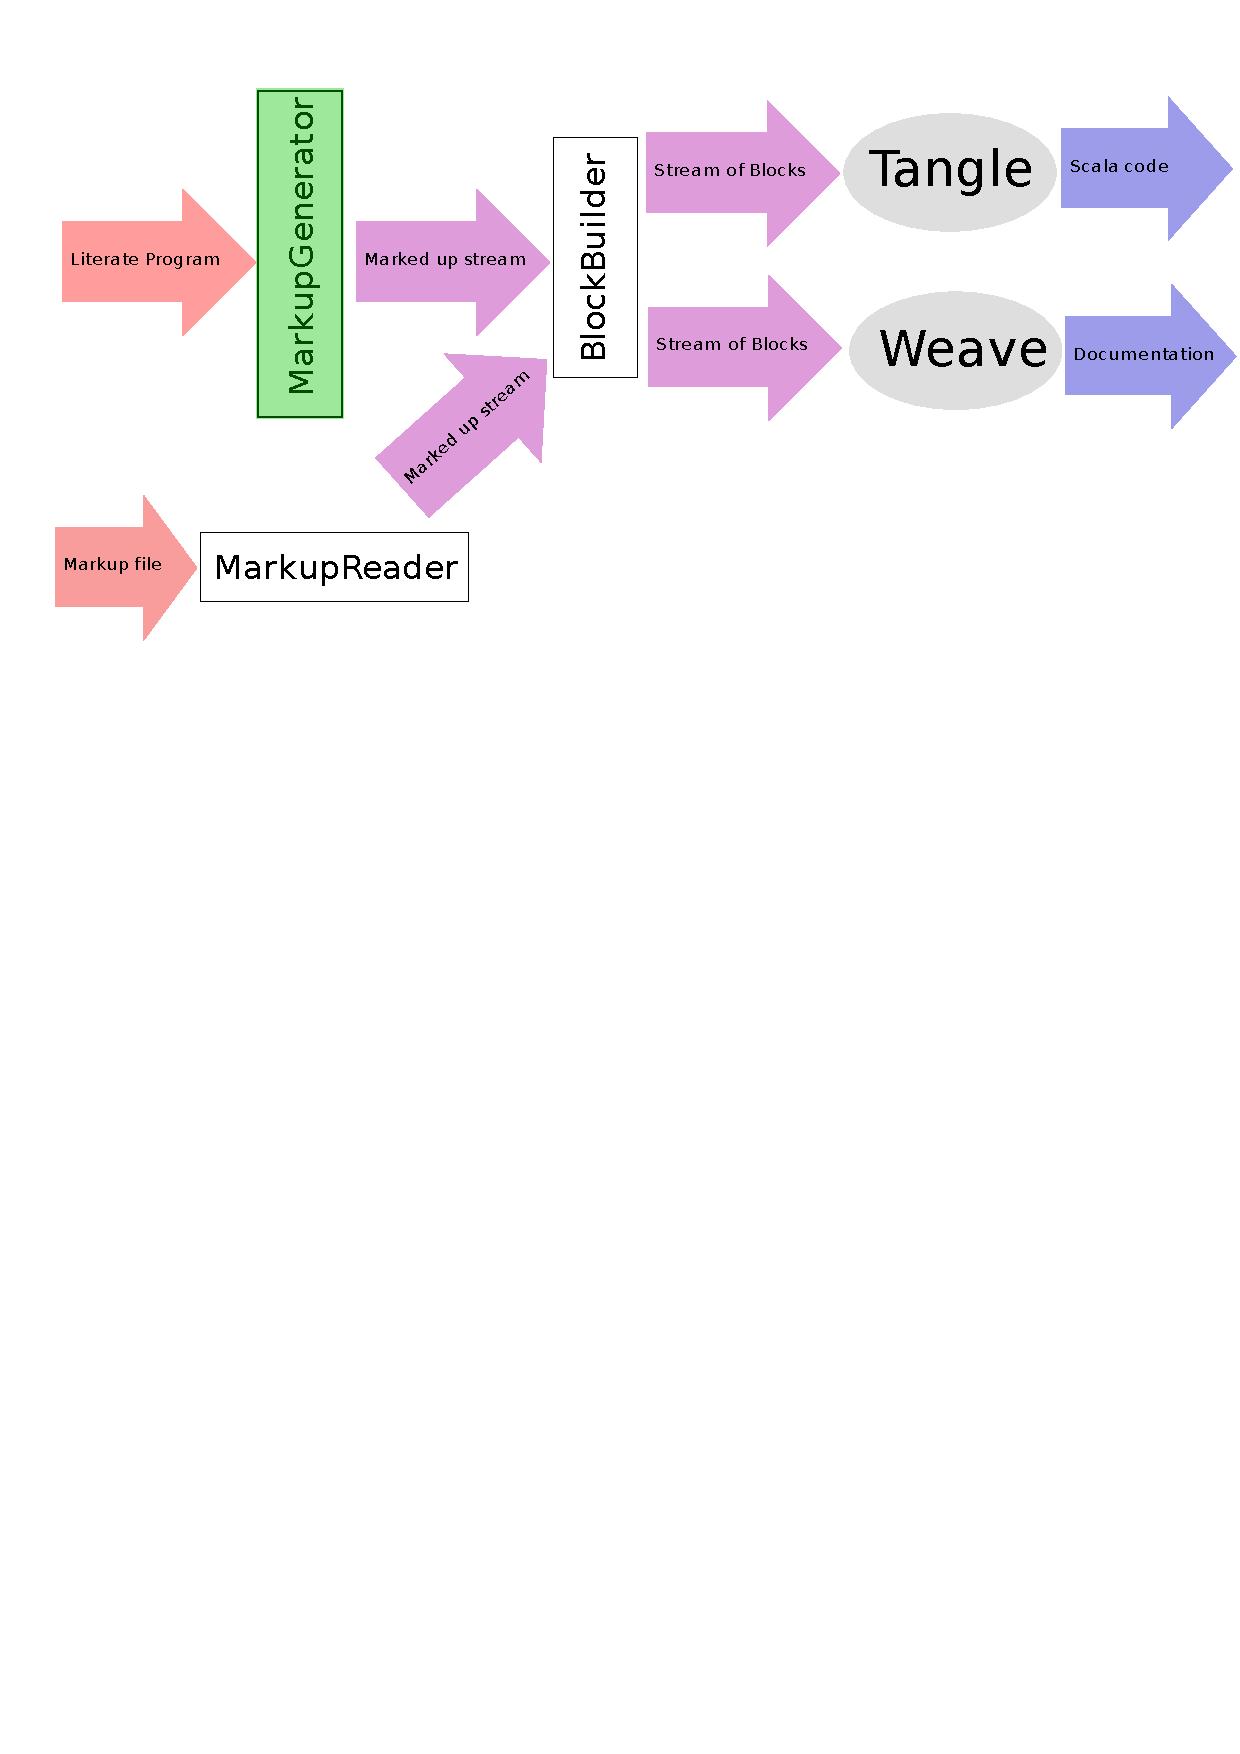
\includegraphics[viewport=0 500 264 800,clip,height=7cm]{images/markupGenerator.pdf}
Now that we know enough about the intermediary format, we are ready to
treat the conversion. The final product will be a stream of markup lines
(like we used them above). The first token will be the filename:

$\left<\mbox{\emph{conversion from noweb to markup}}\right>\equiv$
\begin{program}{\vem class}~MarkupGenerator$($in\,{\rm :}~StreamReader,~filename\,{\rm :}~String$)$~{\small\{}
\\~~~~{\vem def}~lines\,{\rm :}~Stream$[$Line$]$~=
\\~~~~~~~~Stream.cons$($File$($filename$)$,
\\~~~~~~~~Stream.cons$($Doc$($0$)$,documentation$($in,0$)$$)$$)$
\\~~~~$<$in~documentation~mode$>$
\\~~~~$<$in~quote~mode$>$
\\~~~~$<$in~code~mode$>$
\\[0.5em]~~~~$<$read~chunk~name$>$
\\~~~~$<$read~use~name$>$
\\[0.5em]~~~~$<$tab~handling$>$
\\{\small\}}
\\[0.5em]\end{program}\classdefinition{MarkupGenerator}
\methoddefinition{MarkupGenerator}{lines}
\valuedefinition{MarkupGenerator}{in}
\valuedefinition{MarkupGenerator}{filename}



The second token is also already given: The start of the first documentation
block. A noweb file will always start with a block like this. The next section
defines how the documentation mode works.

\subsubsection{The documentation mode}
The documentation mode will accumulate TextLines and NewLines as long as we
do not see a combination that would terminate this documentation chunk:

\begin{itemize}
\item Another documentation chunk (at sign on a new line)
\item A quoted section
\item Beginning of a code block
\end{itemize}

To memorize the line content, we will use an accumulator.

$\left<\mbox{\emph{in documentation mode}}\right>\equiv$
\begin{program}~~~~~~{\vem def}~documentation$($inp\,{\rm :}~StreamReader,
\\~~~~~~~~~~~~~~~~~~~~~~~~~~~~~~~~docnumber\,{\rm :}~Int$)${\rm :}~Stream$[$Line$]$~=~{\small\{}
\\~~~~~~~~~~{\vem def}~docAcc$($input\,{\rm :}~StreamReader,
\\~~~~~~~~~~~~~~~~~~~~~~~~~~acc\,{\rm :}~List$[$Char$]$$)${\rm :}~Stream$[$Line$]$~=
\\~~~~~~~~~~~~~~$<$accumulate~in~doc~mode$>$
\\[0.5em]~~~~~~~~~~docAcc$($inp,Nil$)$
\\~~~~~~{\small\}}
\\[0.5em]\end{program}\methoddefinition{MarkupGenerator}{documentation}



Now let us look at how to produce some lines:

$\left<\mbox{\emph{accumulate in doc mode}}\right>\equiv$
\begin{program}~~input.first~{\vem match}~{\small\{}
\\~~~~~~{\vem case}~'$[$'~$\Rightarrow$~input.rest.first~{\vem match}~{\small\{}
\\~~~~~~~~~~{\vem case}~'$[$'~$\Rightarrow$
\\~~~~~~~~~~~~~~{\vem val}~$($content,continue$)$~=~quote$($input.rest.rest$)$
\\~~~~~~~~~~~~~~acc~{\vem match}~{\small\{}
\\~~~~~~~~~~~~~~~~~~{\vem case}~Nil~$\Rightarrow$
\\~~~~~~~~~~~~~~~~~~~~~~Stream.concat$($
\\~~~~~~~~~~~~~~~~~~~~~~~~~~Stream.cons$($Quote,content$)$,
\\~~~~~~~~~~~~~~~~~~~~~~~~~~Stream.cons$($EndQuote,
\\~~~~~~~~~~~~~~~~~~~~~~~~~~~~~~~~~~~~~~~~~~~~~~docAcc$($continue,Nil$)$$)$$)$
\\~~~~~~~~~~~~~~~~~~{\vem case}~\_~~~$\Rightarrow$
\\~~~~~~~~~~~~~~~~~~~~~~Stream.concat$($
\\~~~~~~~~~~~~~~~~~~~~~~~~~~Stream.cons$($TextLine$($acc.reverse~mkString~""$)$,
\\~~~~~~~~~~~~~~~~~~~~~~~~~~Stream.cons$($Quote,
\\~~~~~~~~~~~~~~~~~~~~~~~~~~~~~~~~~~~~~~~~~~~~content$)$$)$,
\\~~~~~~~~~~~~~~~~~~~~~~~~~~Stream.cons$($EndQuote,
\\~~~~~~~~~~~~~~~~~~~~~~~~~~~~~~~~~~~~~~~~~~~~docAcc$($continue,Nil$)$$)$$)$
\\~~~~~~~~~~~~~~{\small\}}
\\~~~~{\vem case}~\_~$\Rightarrow$~docAcc$($input.rest,~input.first~{\rm :}{\rm :}~acc$)$
\\{\small\}}
\\[0.5em]\end{program}


If we encounter the beginning of a quoted section, then we will call
the quote mode just to continue parsing afterwards. If we encounter the
at sign at the beginning of a line, we will start a new documentation chunk:

$\left<\mbox{\emph{accumulate in doc mode}}\right>+\equiv$
\begin{program}~~{\vem case}~'@'~$\Rightarrow$~acc~{\vem match}~{\small\{}
\\~~~~~~{\vem case}~Nil~$\Rightarrow$
\\~~~~~~~~~~{\vem if}$($~input.rest.first~$==$~'$\backslash$n'~$\,|$$\,|$
\\~~~~~~~~~~~~~~~~~~~~~~~~~~~~~~~~input.rest.first~$==$~'~'~$)$
\\~~~~~~~~~~~~~~Stream.cons$($EndDoc$($docnumber$)$,
\\~~~~~~~~~~~~~~Stream.cons$($Doc$($docnumber~$+$~1$)$,
\\~~~~~~~~~~~~~~~~~~~~~~~~~~~~~~~~documentation$($input.rest.rest,docnumber~$+$~1$)$$)$$)$
\\~~~~~~~~~~{\vem else}
\\~~~~~~~~~~~~~~docAcc$($input.rest,~List$($'@'$)$$)$
\\~~~~~~{\vem case}~\_~$\Rightarrow$~docAcc$($input.rest,~'@'~{\rm :}{\rm :}~acc$)$
\\~~{\small\}}
\\[0.5em]\end{program}


A documentation section can also be terminated by the beginning of a
code chunk. This chunk will be between \texttt{$\langle$$\langle$} and \texttt{$\rangle$$\rangle$=}. If a code
chunk seems to be opened but a newline follows before it was closed,
we have to report this error:

$\left<\mbox{\emph{accumulate in doc mode}}\right>+\equiv$
\begin{program}~~{\vem case}~'$<$'~$\Rightarrow$~input.rest.first~{\vem match}~{\small\{}
\\~~~~~~{\vem case}~'$<$'~$\Rightarrow$~acc~{\vem match}~{\small\{}
\\~~~~~~~~~~{\vem case}~x~{\rm :}{\rm :}~xs~$\Rightarrow$
\\~~~~~~~~~~~~~~~~~~~~~~~~~~~~~~error$($"Unescaped~$<\!$$<$~in~doc~mode"$)$
\\~~~~~~~~~~{\vem case}~Nil~$\Rightarrow$
\\~~~~~~~~~~~~~~~~~~{\vem val}~$($chunkName,continue$)$~=~chunkDef$($input.rest.rest$)$
\\~~~~~~~~~~~~~~~~~~Stream.cons$($EndDoc$($docnumber$)$,
\\~~~~~~~~~~~~~~~~~~Stream.cons$($Code$($docnumber~$+$~1$)$,
\\~~~~~~~~~~~~~~~~~~~~~~code$($continue,chunkName,docnumber$+$1$)$$)$$)$
\\~~~~~~{\small\}}
\\~~~~~~{\vem case}~\_~$\Rightarrow$~docAcc$($input.rest,~'$<$'~{\rm :}{\rm :}~acc$)$
\\~~{\small\}}
\\[0.5em]\end{program}


If we were able to read a chunk name, we will open a new code section
with this information.

$\left<\mbox{\emph{accumulate in doc mode}}\right>+\equiv$
\begin{program}~~{\vem case}~c~$\Rightarrow$
\\~~~~~~{\vem if}$($~c~$==$~'$\backslash$n'~$)$~{\small\{}
\\~~~~~~~~~~Stream.cons$($TextLine$($acc.reverse~mkString~""$)$,
\\~~~~~~~~~~Stream.cons$($NewLine,docAcc$($input.rest,Nil$)$$)$$)$
\\~~~~~~{\small\}}~{\vem else}~{\small\{}
\\~~~~~~~~~~{\vem if}$($~!input.atEnd~$)$~docAcc$($input.rest,input.first~{\rm :}{\rm :}~acc$)$
\\~~~~~~~~~~{\vem else}~acc~{\vem match}~{\small\{}
\\~~~~~~~~~~~~~~{\vem case}~Nil~$\Rightarrow$~Stream.cons$($EndDoc$($docnumber$)$,
\\~~~~~~~~~~~~~~~~~~~~~~~~~~~~~~~~~~~~~~~~~~~~~~~~~~~~~~~~~~Stream.empty$)$
\\~~~~~~~~~~~~~~{\vem case}~\_~$\Rightarrow$
\\~~~~~~~~~~~~~~~~~~Stream.cons$($TextLine$($acc.reverse~mkString~""$)$,
\\~~~~~~~~~~~~~~~~~~Stream.cons$($NewLine,
\\~~~~~~~~~~~~~~~~~~Stream.cons$($EndDoc$($docnumber$)$,Stream.empty$)$$)$$)$
\\~~~~~~~~~~{\small\}}
\\~~~~~~{\small\}}
\\~~{\small\}}
\\[0.5em]\end{program}


As a general rule, all markup files will have a newline at the end. If
no newline is there, then we will add one.

\subsubsection{The quote mode}
In quote mode, we will ignore all normal control characters up until the
point where we encounter the close quote \texttt{]]}. Note, however, that additional
\texttt{]}s have to be taken into account: The quote is only closed with the
last \texttt{]} in a row.

$\left<\mbox{\emph{in quote mode}}\right>\equiv$
\begin{program}{\vem def}~quote$($inp\,{\rm :}~StreamReader$)${\rm :}~$($Stream$[$Line$]$,~StreamReader$)$~=~{\small\{}
\\~~~~{\vem def}~quoteAcc$($input\,{\rm :}~StreamReader,~acc\,{\rm :}~List$[$Char$]$$)${\rm :}
\\~~~~~~~~~~$($Stream$[$Line$]$,~StreamReader$)$~=
\\~~input.first~{\vem match}~{\small\{}
\\~~~~~~{\vem case}~'$]$'~$\Rightarrow$~input.rest.first~{\vem match}~{\small\{}
\\~~~~~~~~~~{\vem case}~'$]$'~$\Rightarrow$~input.rest.rest.first~{\vem match}~{\small\{}
\\~~~~~~~~~~~~~~{\vem case}~'$]$'~$\Rightarrow$~quoteAcc$($input.rest,'$]$'~{\rm :}{\rm :}~acc$)$
\\~~~~~~~~~~~~~~{\vem case}~\_~$\Rightarrow$~acc~{\vem match}~{\small\{}
\\~~~~~~~~~~~~~~~~~~{\vem case}~Nil~$\Rightarrow$~$($Stream.empty,input.rest.rest$)$
\\~~~~~~~~~~~~~~~~~~{\vem case}~\_~$\Rightarrow$~$($Stream.cons$($TextLine$($acc.reverse~mkString~""$)$,
\\~~~~~~~~~~~~~~~~~~~~~~~~~~~~~~~~~~~~~~~~~~~~~~~~~~~~~~~~~~~~~~~~Stream.empty$)$,
\\~~~~~~~~~~~~~~~~~~~~~~~~~~~~~~~~~~~~~~~~input.rest.rest$)$
\\~~~~~~~~~~~~~~{\small\}}
\\~~~~~~~~~~{\small\}}
\\~~~~~~~~~~{\vem case}~\_~$\Rightarrow$~quoteAcc$($input.rest,'$]$'~{\rm :}{\rm :}~acc$)$
\\~~~~~~{\small\}}
\\~~~~~~{\vem case}~'$\backslash$n'~$\Rightarrow$~acc~{\vem match}~{\small\{}
\\~~~~~~~~~~{\vem case}~Nil~$\Rightarrow$~{\vem val}~$($more,contreader$)$~=~quoteAcc$($input.rest,Nil$)$
\\~~~~~~~~~~~~~~~~~~~~~~~~~~~~~~~~~~$($Stream.cons$($NewLine,more$)$,contreader$)$
\\~~~~~~~~~~{\vem case}~\_~$\Rightarrow$~{\vem val}~$($more,contreader$)$~=~quoteAcc$($input.rest,Nil$)$
\\~~~~~~~~~~~~~~~~~~~~~~~~~~~~~~$($Stream.cons$($TextLine$($acc.reverse~mkString~""$)$,
\\~~~~~~~~~~~~~~~~~~~~~~~~~~~~~~Stream.cons$($NewLine,~more$)$$)$,contreader$)$
\\~~~~~~{\small\}}
\\~~~~~~{\vem case}~c~$\Rightarrow$~quoteAcc$($input.rest,~c~{\rm :}{\rm :}~acc$)$
\\~~{\small\}}
\\~~~~~~~~~~~~~~quoteAcc$($inp,Nil$)$
\\{\small\}}
\\[0.5em]\end{program}\methoddefinition{MarkupGenerator}{quote}



\subsubsection{The code mode}
Code chunks are a bit different from documentation chunks in the fact that
they are named. The following method reads the name of a documentation chunk
and returns it:

$\left<\mbox{\emph{read chunk name}}\right>\equiv$
\begin{program}{\vem def}~chunkDef$($inp\,{\rm :}~StreamReader$)${\rm :}~$($String,~StreamReader$)$~=~{\small\{}
\\~~~~{\vem def}~chunkAcc$($input\,{\rm :}~StreamReader,~acc\,{\rm :}~List$[$Char$]$$)${\rm :}
\\~~~~$($String,~StreamReader$)$~=
\\~~~~input.first~{\vem match}~{\small\{}
\\~~~~~~~~{\vem case}~'$>$'~$\Rightarrow$~input.rest.first~{\vem match}~{\small\{}
\\~~~~~~~~~~~~{\vem case}~'$>$'~$\Rightarrow$~input.rest.rest.first~{\vem match}~{\small\{}
\\~~~~~~~~~~~~{\vem case}~'='~$\Rightarrow$~$($$($acc.reverse~mkString~""$)$,input.rest.rest.rest$)$
\\~~~~~~~~~~~~{\vem case}~\_~$\Rightarrow$~System.err.println$($"Unescaped"$)$;~exit
\\~~~~~~~~{\small\}}
\\~~~~~~~~{\vem case}~\_~$\Rightarrow$~chunkAcc$($input.rest,~'$>$'~{\rm :}{\rm :}~acc$)$
\\~~~~{\small\}}
\\~~~~{\vem case}~c~$\Rightarrow$~chunkAcc$($input.rest,~c~{\rm :}{\rm :}~acc$)$
\\~~~~{\small\}}
\\[0.5em]~~~~chunkAcc$($inp,~Nil$)$
\\{\small\}}
\\[0.5em]\end{program}\methoddefinition{MarkupGenerator}{chunkDef}



Now that we know how we can read in the chunk name, let us look on how to
read code sections:

$\left<\mbox{\emph{in code mode}}\right>\equiv$
\begin{program}{\vem def}~code$($inp\,{\rm :}~StreamReader,~chunkname\,{\rm :}~String,~codenumber\,{\rm :}~Int$)${\rm :}
\\~~~~Stream$[$Line$]$~=~{\small\{}
\\~~~~~~$<$detect~{\vem new}~code~chunk$>$
\\~~~~~~$<$detect~{\vem new}~use~directive$>$
\\~~~~{\vem def}~codeAcc$($input\,{\rm :}~StreamReader,~acc\,{\rm :}~List$[$Char$]$$)${\rm :}
\\~~~~~~~~Stream$[$Line$]$~=~input.first~{\vem match}~{\small\{}
\\~~~~~~~~~~~~{\vem case}~'$<$'~$\Rightarrow$~input.rest.first~{\vem match}~{\small\{}
\\~~~~~~~~~~~~~~~~{\vem case}~'$<$'~$\Rightarrow$
\\~~~~~~~~~~~~~~~~~~~~acc~{\vem match}~{\small\{}
\\~~~~~~~~~~~~~~~~~~~~~~~~{\vem case}~Nil~$\Rightarrow$
\\~~~~~~~~~~~~~~~~~~~~~~~~{\vem if}$($~isNewCodeChunk$($input.rest.rest$)$~$)$~{\small\{}
\\~~~~~~~~~~~~~~~~~~~~~~~~~~~~{\vem val}~$($chunkName,continue$)$~=
\\~~~~~~~~~~~~~~~~~~~~~~~~~~~~~~~~chunkDef$($input.rest.rest$)$
\\~~~~~~~~~~~~~~~~~~~~~~~~~~~~Stream.cons$($EndCode$($codenumber$)$,
\\~~~~~~~~~~~~~~~~~~~~~~~~~~~~Stream.cons$($Code$($codenumber~$+$~1$)$,
\\~~~~~~~~~~~~~~~~~~~~~~~~~~~~~~~~code$($continue,
\\~~~~~~~~~~~~~~~~~~~~~~~~~~~~~~~~chunkName,
\\~~~~~~~~~~~~~~~~~~~~~~~~~~~~~~~~codenumber~$+$~1$)$$)$$)$
\\~~~~~~~~~~~~~~~~~~~~~~~~{\small\}}~{\vem else}~{\vem if}$($~isNewUseDirective$($input.rest$)$~$)$~{\small\{}
\\~~~~~~~~~~~~~~~~~~~~~~~~~~~~{\vem val}~$($usename,cont$)$~=~use$($input.rest.rest$)$
\\~~~~~~~~~~~~~~~~~~~~~~~~~~~~Stream.cons$($Use$($usename$)$,
\\~~~~~~~~~~~~~~~~~~~~~~~~~~~~~~~~~~~~codeAcc$($cont,Nil$)$$)$
\\~~~~~~~~~~~~~~~~~~~~~~~~{\small\}}~{\vem else}~{\small\{}
\\~~~~~~~~~~~~~~~~~~~~~~~~~~~~codeAcc$($input.rest,'$<$'~{\rm :}{\rm :}~acc$)$
\\~~~~~~~~~~~~~~~~~~~~~~~~{\small\}}
\end{program}\methoddefinition{MarkupGenerator}{code}



If we are not at the beginning of a line (\texttt{acc} is not empty), then
we don't have to worry about new code chunks, just use directives:

$\left<\mbox{\emph{in code mode}}\right>+\equiv$
\begin{program}~~~~~~~~~~~~~~~~~~~~~~~~{\vem case}~\_~$\Rightarrow$
\\~~~~~~~~~~~~~~~~~~~~~~~~{\vem if}$($~isNewUseDirective$($input.rest$)$~$)$~{\small\{}
\\~~~~~~~~~~~~~~~~~~~~~~~~~~~~{\vem val}~$($usename,cont$)$~=~use$($input.rest.rest$)$
\\~~~~~~~~~~~~~~~~~~~~~~~~~~~~Stream.cons$($TextLine$($acc.reverse~mkString~""$)$,
\\~~~~~~~~~~~~~~~~~~~~~~~~~~~~Stream.cons$($Use$($usename$)$,
\\~~~~~~~~~~~~~~~~~~~~~~~~~~~~~~~~codeAcc$($cont,~Nil$)$$)$$)$
\\~~~~~~~~~~~~~~~~~~~~~~~~{\small\}}~{\vem else}~{\small\{}
\\~~~~~~~~~~~~~~~~~~~~~~~~~~~~codeAcc$($input.rest,~'$<$'~{\rm :}{\rm :}~acc$)$
\\~~~~~~~~~~~~~~~~~~~~~~~~{\small\}}
\\~~~~~~~~~~~~~~~~~~~~{\small\}}
\\~~~~~~~~~~~~~~~~~~~~{\vem case}~\_~$\Rightarrow$~codeAcc$($input.rest,~'$<$'~{\rm :}{\rm :}~acc$)$
\\~~~~~~~~~~~~~~~~{\small\}}
\\[0.5em]\end{program}


In a code section, we might also encounter \texttt{$\langle$$\langle$}. But here, it might either
be the beginning of a new code section or a use directive: Unfortunately,
we can't know without scanning ahead, so we use our little utility
function \texttt{isNewCodeChunk}:

$\left<\mbox{\emph{detect new code chunk}}\right>\equiv$
\begin{program}~~~~~~~~~~{\vem def}~isNewCodeChunk$($input\,{\rm :}~StreamReader$)${\rm :}~Boolean~=
\\~~~~~~~~~~~~~~input.first~{\vem match}~{\small\{}
\\~~~~~~~~~~~~~~~~~~{\vem case}~'$>$'~$\Rightarrow$~input.rest.first~{\vem match}~{\small\{}
\\~~~~~~~~~~~~~~~~~~~~~~{\vem case}~'$>$'~$\Rightarrow$~input.rest.rest.first~{\vem match}~{\small\{}
\\~~~~~~~~~~~~~~~~~~~~~~~~~~{\vem case}~'='~$\Rightarrow$~{\vem true}
\\~~~~~~~~~~~~~~~~~~~~~~~~~~{\vem case}~\_~$\Rightarrow$~{\vem false}
\\~~~~~~~~~~~~~~~~~~~~~~{\small\}}
\\~~~~~~~~~~~~~~~~~~~~~~{\vem case}~\_~$\Rightarrow$~isNewCodeChunk$($input.rest$)$
\\~~~~~~~~~~~~~~~~~~{\small\}}
\\~~~~~~~~~~~~~~~~~~{\vem case}~c~$\Rightarrow$
\\~~~~~~~~~~~~~~~~~~~~~~{\vem if}$($~c~$==$~'$\backslash$n'~$)$
\\~~~~~~~~~~~~~~~~~~~~~~~~~~{\vem false}
\\~~~~~~~~~~~~~~~~~~~~~~{\vem else}~isNewCodeChunk$($input.rest$)$
\\~~~~~~~~~~{\small\}}
\\[0.5em]\end{program}


To detect whether we are treating a new use directive is very similiar:

$\left<\mbox{\emph{detect new use directive}}\right>\equiv$
\begin{program}~~~~~~~~~~{\vem def}~isNewUseDirective$($input\,{\rm :}~StreamReader$)${\rm :}~Boolean~=
\\~~~~~~~~~~input.first~{\vem match}~{\small\{}
\\~~~~~~~~~~~~~~{\vem case}~'$>$'~$\Rightarrow$~input.rest.first~{\vem match}~{\small\{}
\\~~~~~~~~~~~~~~~~~~{\vem case}~'$>$'~$\Rightarrow$~input.rest.rest.first~{\vem match}~{\small\{}
\\~~~~~~~~~~~~~~~~~~~~~~{\vem case}~'='~$\Rightarrow$~{\vem false}
\\~~~~~~~~~~~~~~~~~~~~~~{\vem case}~\_~~~$\Rightarrow$~{\vem true}
\\~~~~~~~~~~~~~~~~~~{\small\}}
\\~~~~~~~~~~~~~~~~~~{\vem case}~\_~$\Rightarrow$~isNewUseDirective$($input.rest$)$
\\~~~~~~~~~~~~~~{\small\}}
\\~~~~~~~~~~~~~~{\vem case}~c~$\Rightarrow$
\\~~~~~~~~~~~~~~~~~~{\vem if}$($~c~$==$~'$\backslash$n'~$)$~{\vem false}
\\~~~~~~~~~~~~~~~~~~{\vem else}~isNewUseDirective$($input.rest$)$
\\~~~~~~~~~~{\small\}}
\\[0.5em]\end{program}


This can tell us whether we really have a new code chunk before us,
but not whether we really have a use directive.

A code block is also finished upon seeing an at sign:

$\left<\mbox{\emph{in code mode}}\right>+\equiv$
\begin{program}{\vem case}~'@'~$\Rightarrow$
\\~~~~{\vem if}$($~input.rest.first~$==$~'~'~$\,|$$\,|$
\\~~~~~~~~~~input.rest.first~$==$~'$\backslash$n'~$)$
\\~~~~~~~~acc~{\vem match}~{\small\{}
\\~~~~~~~~~~~~{\vem case}~Nil~$\Rightarrow$~Stream.cons$($EndCode$($codenumber$)$,
\\~~~~~~~~~~~~~~~~~~~~~~~~~~~~~~~~~~~~Stream.cons$($Doc$($codenumber~$+$~1$)$,
\\~~~~~~~~~~~~~~~~~~~~~~~~~~~~~~~~~~~~documentation$($input.rest.rest,
\\~~~~~~~~~~~~~~~~~~~~~~~~~~~~~~~~~~~~~~~~~~~~~~~~~~~~~~~~~~~~~~~~codenumber~$+$~1$)$$)$$)$
\\~~~~~~~~~~~~{\vem case}~\_~$\Rightarrow$~codeAcc$($input.rest,~'@'~{\rm :}{\rm :}~acc$)$
\\~~~~~~~~{\small\}}
\\~~~~{\vem else}~codeAcc$($input.rest,~'@'~{\rm :}{\rm :}~acc$)$
\\[0.5em]\end{program}


If none of these special cases occurred, we can simply continue parsing
lines.

$\left<\mbox{\emph{in code mode}}\right>+\equiv$
\begin{program}{\vem case}~c~$\Rightarrow$
\\~~~~{\vem if}$($~c~$==$~'$\backslash$n'~$)$~{\small\{}
\\~~~~~~~~{\vem val}~tl~=~TextLine$($acc.reverse~mkString~""$)$
\\~~~~~~~~Stream.cons$($tl,
\\~~~~~~~~Stream.cons$($NewLine,codeAcc$($input.rest,Nil$)$$)$$)$
\\[0.5em]\end{program}


This newline thing is quite peculiar: If we encounter two newlines
without any text in between, we will still interleave an empty text node.

$\left<\mbox{\emph{in code mode}}\right>+\equiv$
\begin{program}~~~~{\small\}}~{\vem else}~{\small\{}
\\~~~~~~~~{\vem if}$($~input.atEnd~$)$
\\~~~~~~~~~~~~acc~{\vem match}~{\small\{}
\\~~~~~~~~~~~~~~~~{\vem case}~Nil~$\Rightarrow$~Stream.cons$($EndCode$($codenumber$)$,
\\~~~~~~~~~~~~~~~~~~~~~~~~~~~~~~~~~~~~~~~~~~~~~~~~~~~~~~~~~~~~~~~~Stream.empty$)$
\\~~~~~~~~~~~~~~~~{\vem case}~\_~$\Rightarrow$
\\~~~~~~~~~~~~~~~~~~~~Stream.cons$($TextLine$($acc.reverse~mkString~""$)$,
\\~~~~~~~~~~~~~~~~~~~~Stream.cons$($NewLine,
\\~~~~~~~~~~~~~~~~~~~~Stream.cons$($EndCode$($codenumber$)$,Stream.empty$)$$)$$)$
\\~~~~~~~~~~~~{\small\}}
\\~~~~~~~~{\vem else}~{\vem if}$($~c~$==$~'$\backslash$t'~$)$
\\~~~~~~~~~~~~codeAcc$($input.rest,tab~{\rm :}{\rm :}{\rm :}~acc~$)$
\\~~~~~~~~{\vem else}
\\~~~~~~~~~~~~codeAcc$($input.rest,c~{\rm :}{\rm :}~acc~$)$
\\~~~~{\small\}}
\\{\small\}}
\\~~~~~~~~
\\Stream.cons$($Definition$($chunkname$)$,
\\Stream.cons$($NewLine,
\\~~~~~~~~~~~~~~~~codeAcc$($inp.rest,Nil$)$$)$$)$
\\{\small\}}
\\[0.5em]\end{program}


A little strangeness comes from the tab character: markup expands this character
to eight spaces, so we'll do that too:

$\left<\mbox{\emph{tab handling}}\right>\equiv$
\begin{program}~~~~{\vem val}~tab~=~$($1~to~8~map~{\small\{}~x~$\Rightarrow$~'~'~{\small\}}$)$.toList
\\[0.5em]\end{program}


\subsubsection{Reading a use name}
There is still a small utility function missing: the one to read which
chunk to use:

$\left<\mbox{\emph{read use name}}\right>\equiv$
\begin{program}~~~~{\vem def}~use$($inp\,{\rm :}~StreamReader$)${\rm :}~$($String,~StreamReader$)$~=~{\small\{}
\\~~~~~~~~{\vem def}~useAcc$($input\,{\rm :}~StreamReader,~acc\,{\rm :}~List$[$Char$]$$)${\rm :}
\\~~~~~~~~~~~~~~~~~~~~$($String,StreamReader$)$~=~input.first~{\vem match}~{\small\{}
\\~~~~~~~~~~~~{\vem case}~'$>$'~$\Rightarrow$~input.rest.first~{\vem match}~{\small\{}
\\~~~~~~~~~~~~~~~~{\vem case}~'$>$'~$\Rightarrow$~$($acc.reverse~mkString~"",input.rest.rest$)$
\\~~~~~~~~~~~~~~~~{\vem case}~\_~$\Rightarrow$~useAcc$($input.rest,~'$>$'~{\rm :}{\rm :}~acc$)$
\\~~~~~~~~~~~~{\small\}}
\\~~~~~~~~~~~~{\vem case}~c~$\Rightarrow$~useAcc$($input.rest,~c~{\rm :}{\rm :}~acc$)$
\\~~~~~~~~{\small\}}
\\[0.5em]~~~~~~~~useAcc$($inp,Nil$)$
\\~~~~{\small\}}
\\[0.5em]
\end{program}\methoddefinition{MarkupGenerator}{use}



\subsection{The command line application}
As we have seen, the data structures produced during the markup step can
be directly used by further stages. To gain some compatibility with noweb
(and access to other filters provided by it), we can also output the
intermediary format. This will be done when we call the application
\texttt{Markup}. We use the literate settings defined in \texttt{util/commandline.nw}

$\left<\mbox{\emph{markup generator}}\right>\equiv$
\begin{program}{\vem object}~Markup~{\small\{}
\\[0.5em]~~~~{\vem def}~usage\,{\rm :}~Unit~=~{\small\{}
\\~~~~~~~~System.err.println$($"Usage\,{\rm :}~scala~markup.Markup~$[$infile$]$$\backslash$n"$)$
\\~~~~{\small\}}
\\[0.5em]~~~~{\vem def}~main$($args\,{\rm :}~Array$[$String$]$$)$~=~{\small\{}
\\~~~~~~~~{\vem import}~util.LiterateSettings
\\[0.5em]~~~~~~~~{\vem val}~settings~=~{\vem new}~LiterateSettings$($args$)$
\\[0.5em]~~~~~~~~{\vem val}~listlines\,{\rm :}~List$[$Stream$[$Line$]$$]$~=~settings.lines
\\~~~~~~~~listlines~foreach~{\small\{}
\\~~~~~~~~~~~~linestream~$\Rightarrow$~linestream~foreach~println
\\~~~~~~~~{\small\}}
\\~~~~{\small\}}
\\{\small\}}
\end{program}\objectdefinition{Markup}
\methoddefinition{Markup}{usage}
\methoddefinition{Markup}{main}



\end{document}


